\chapter{Viaje de Investigación}
\label{cp:europe-trip}

Durante la ejecución de este trabajo de tesis, el proceso de investigación fue complementado por una experiencia de campo que, aunque ajena a la planificación inicial, resultó ser enriquecedora para el trabajo. En noviembre de 2024, se realizó un viaje de investigación a Europa con el objetivo de estudiar de primera mano los sistemas de reciclaje y los modelos de \gls{economiacircular} implementados en diversas ciudades. Esta oportunidad permitió obtener una perspectiva global que, si bien generó un desvío en el cronograma, aportó un conocimiento valioso y una visión práctica de los desafíos abordados en este trabajo.

La experiencia, de dos semanas de duración, incluyó visitas a centros de reciclaje, interacciones con organizaciones dedicadas a la \gls{sostenibilidad} y el estudio de redes de comercio circular en tres ciudades: Madrid (España), Ámsterdam (Países Bajos) y Berlín (Alemania). Cada una ofreció un panorama distinto de los esfuerzos por promover la economía circular. La primera ciudad visitada fue Madrid, donde se observó la mecánica de la recolección diferenciada y las categorías de residuos en origen. A pesar de que la sociedad española manifiesta un creciente interés por la sostenibilidad, se constató que la implementación de sistemas de reciclaje y economía circular se encuentra en una etapa de desarrollo inicial, en comparación con las ciudades visitadas posteriormente. Se analizó el rol de Ecoembes \footnote{\url{https://www.ecoembes.com/es}}, una organización sin fines de lucro encargada de la gestión de los envases domésticos, cuyo modelo de financiamiento a través de las empresas envasadoras permite costear el proceso de reciclaje. A pesar de su importancia, existen controversias sobre las cifras de reciclaje que reportan y destino final del plástico que gestionan, un debate que pone de manifiesto la complejidad de la medición y regulación en estos sistemas \footnote{Fuente: \url{https://es.greenpeace.org/es/sala-de-prensa/comunicados/ecoembes-miente/}}.

El viaje continuó en Ámsterdam, una ciudad reconocida por su alto nivel de conciencia ambiental y sus esfuerzos por fomentar hábitos de vida sostenibles. Al aterrizar en el aeropuerto de la ciudad se pudo ver un gran parque de energía eólica desde las alturas, una muestra inicial del compromiso de la ciudad con las energías limpias. Se observó el uso extendido de bicicletas y un sistema de transporte público mayoritariamente eléctrico que contribuyen a reducir la huella de carbono de sus habitantes. En la Figura \ref{fig:europe-pictures}.A, se puede observar un estacionamiento de bicicletas repleto en la ciudad de Ámsterdam, un escenario frecuente en toda la ciudad. En lo que respecta al reciclaje de envases, Ámsterdam implementa un \acrfull{drs}, en el que los consumidores pagan un depósito por botellas y latas, el cual es reembolsado al devolver los envases en máquinas \acrshort{rvm} (\acrfull{rvm}) ubicadas en los supermercados. Este sistema ha demostrado ser efectivo para aumentar las tasas de reciclaje de envases. Sin embargo, se identificó un problema de higiene pública, donde los contenedores de basura en la vía pública son vandalizados por recolectores informales que buscan los envases desechados para obtener el depósito al devolverlos. En la Figura \ref{fig:europe-pictures}.B, se puede observar una fotografía capturada en la vía pública de un contenedor de residuos vandalizado en este contexto. A pesar de esta situación, el sistema ha logrado fomentar el hábito de reciclaje en los ciudadanos. En esta ciudad se visitó un centro verde, donde se constató una alta tasa de recuperación y reciclaje que no se limita a los envases, sino que se extiende a otros residuos como muebles, ropa y madera, entre otros. La separación de residuos es una práctica normal en la rutina de los ciudadanos, que acuden a estos centros para entregar sus residuos y elementos en desuso. Sin embargo, en el servicio de recolección diferenciada semanal, los residentes reclaman que la frecuencia es insuficiente, lo que lleva a que los contenedores se desborden con frecuencia. Por otro lado, al indagar en el destino final de los materiales reciclables, se informó que la mayoría son procesados en el país, pero se desconoce el destino final de aquellos que son exportados fuera de Europa. Además, aunque se encontraron numerosas tiendas de productos sostenibles, se admitió que la \gls{trazabilidad} de los materiales reciclados es limitada, lo que sugiere que la separación de residuos y la venta de productos reciclados son flujos independientes y sin conexión directa.

La última parada del viaje fue Berlín, donde se encontró la cultura de sostenibilidad más avanzada entre las ciudades visitadas. La experiencia comenzó con una reunión con la organización Circular Berlin \footnote{\url{https://circular.berlin/}}, una iniciativa que promueve la economía circular en la región a través de la colaboración entre múltiples actores. Su modelo opera como un punto de encuentro que conecta a emprendimientos, empresas, investigadores, ciudadanos y el gobierno local. El objetivo central de la organización es crear una red de actores para compartir conocimientos, debatir ideas e impulsar proyectos de economía circular, con el fin de catalizar un cambio a nivel comunitario y generar un impacto positivo a nivel cultural, económico y ecológico. En este encuentro, un miembro de la organización presentó su misión y destacó proyectos de circularidad que se estaban desarrollando en Berlín, lo que sirvió como una guía estratégica para organizar las visitas a los diferentes puntos de interés durante la estadía. Este encuentro fue un punto de inflexión en el viaje, proporcionando una hoja de ruta para visitar proyectos específicos y comprender la visión integral de la economía circular en la región, mientras que se exploró cómo la colaboración puede ser un motor de cambio.

En la capital alemana, se observó un sistema \acrshort{drs} similar al de Ámsterdam, pero con diferencias importantes. En Berlín, los consumidores también pagan un depósito por las botellas y latas, el cual es reembolsado al devolver los envases en máquinas \acrshort{rvm} ubicadas en supermercados. En la Figura \ref{fig:europe-pfand-cases}.C se puede observar una fotografía de una máquina \acrshort{rvm} ubicada en el exterior de un supermercado en la ciudad de Berlín. A su vez, en esta ciudad se realizó el experimento de devolver envases en una máquina \acrshort{rvm}, lo que permitió observar de primera mano la experiencia del usuario del sistema PFAND. La Figura \ref{fig:europe-pfand-cases}.A muestra una fotografía de la pantalla de una máquina \acrshort{rvm} en la que se indica un caso de uso inválido en idioma alemán, donde se explica al usuario que la máquina no acepta envases que contienen líquido dentro, mientras que el mensaje de la fotografía \ref{fig:europe-pfand-cases}.B indica que el envase no es aceptado por estar dañado de modo que la máquina no puede reconocerlo, y la Figura \ref{fig:europe-pfand-cases}.C muestra un mensaje que indica que el envase no es aceptado porque no pertenece al sistema PFAND y debe desecharse en un contenedor común por tratarse de un envase importado de otro país o de una marca no registrada en el sistema. Estas situaciones evidencian las limitaciones del sistema actual, donde ciertos envases no son aceptados por las máquinas, lo que puede generar frustración en los usuarios y reducir la efectividad del sistema \acrshort{drs}. 

En el caso de Berlín, a diferencia de Ámsterdam, la conciencia de los ciudadanos ha evolucionado de manera tal que, al desechar envases en la vía pública, prefieren dejarlos junto a los cestos de basura para facilitar que las personas sin hogar los recuperen y obtengan el depósito para adquirir alimentos diariamente con estos fondos. Esta práctica demuestra cómo una iniciativa de reciclaje puede también promover un comportamiento social positivo, evitando los problemas de higiene que se observaron en los Países Bajos. Se visitó un centro verde, similar al de Ámsterdam, donde se reciben y clasifican los residuos. El gran flujo de ciudadanos que acuden a estos centros demuestra el alto compromiso de la población con la reducción y la separación de residuos. A su vez, los trabajadores indicaron que esta es una práctica habitual, ya que los ciudadanos pueden ser multados por dejar grandes volúmenes de residuos en la vía pública. Se identificó, además, una gran presencia de tiendas de segunda mano y comercios circulares que promueven la reutilización y la reducción de residuos. Incluso se visitó una tienda de productos a granel, donde los clientes llevan sus propios envases reutilizables para comprar alimentos y productos de limpieza. A partir de lo observado, se pudo constatar que la economía circular en Berlín está profundamente integrada en la rutina diaria de sus habitantes.

En retrospectiva, el viaje de investigación a Europa resultó ser una experiencia valiosa. Cada ciudad visitada proporcionó una visión única de los desafíos y éxitos de los sistemas de reciclaje y economía circular. Se puede inferir que el sistema \acrshort{drs} es un método que ha demostrado ser efectivo para fomentar el reciclaje de envases, logrando tasas de recuperación superiores al 90\%, un nivel que no se ha alcanzado con otros enfoques \cite{picuno2025potential}. A su vez, se pudo constatar que la conciencia ciudadana es un factor que influye en el éxito de cualquier sistema de reciclaje. Los modelos de colaboración y fomento de proyectos, como los observados en Berlín, son un vehículo eficaz para impulsar la economía circular a nivel regional. El conocimiento obtenido en este viaje apoya la hipótesis de que una solución de trazabilidad del vidrio puede contribuir no solo a la transparencia de la cadena de valor, sino también a generar conciencia y un impacto positivo en la cultura local.

\begin{figure}[!htb]
	\centering
	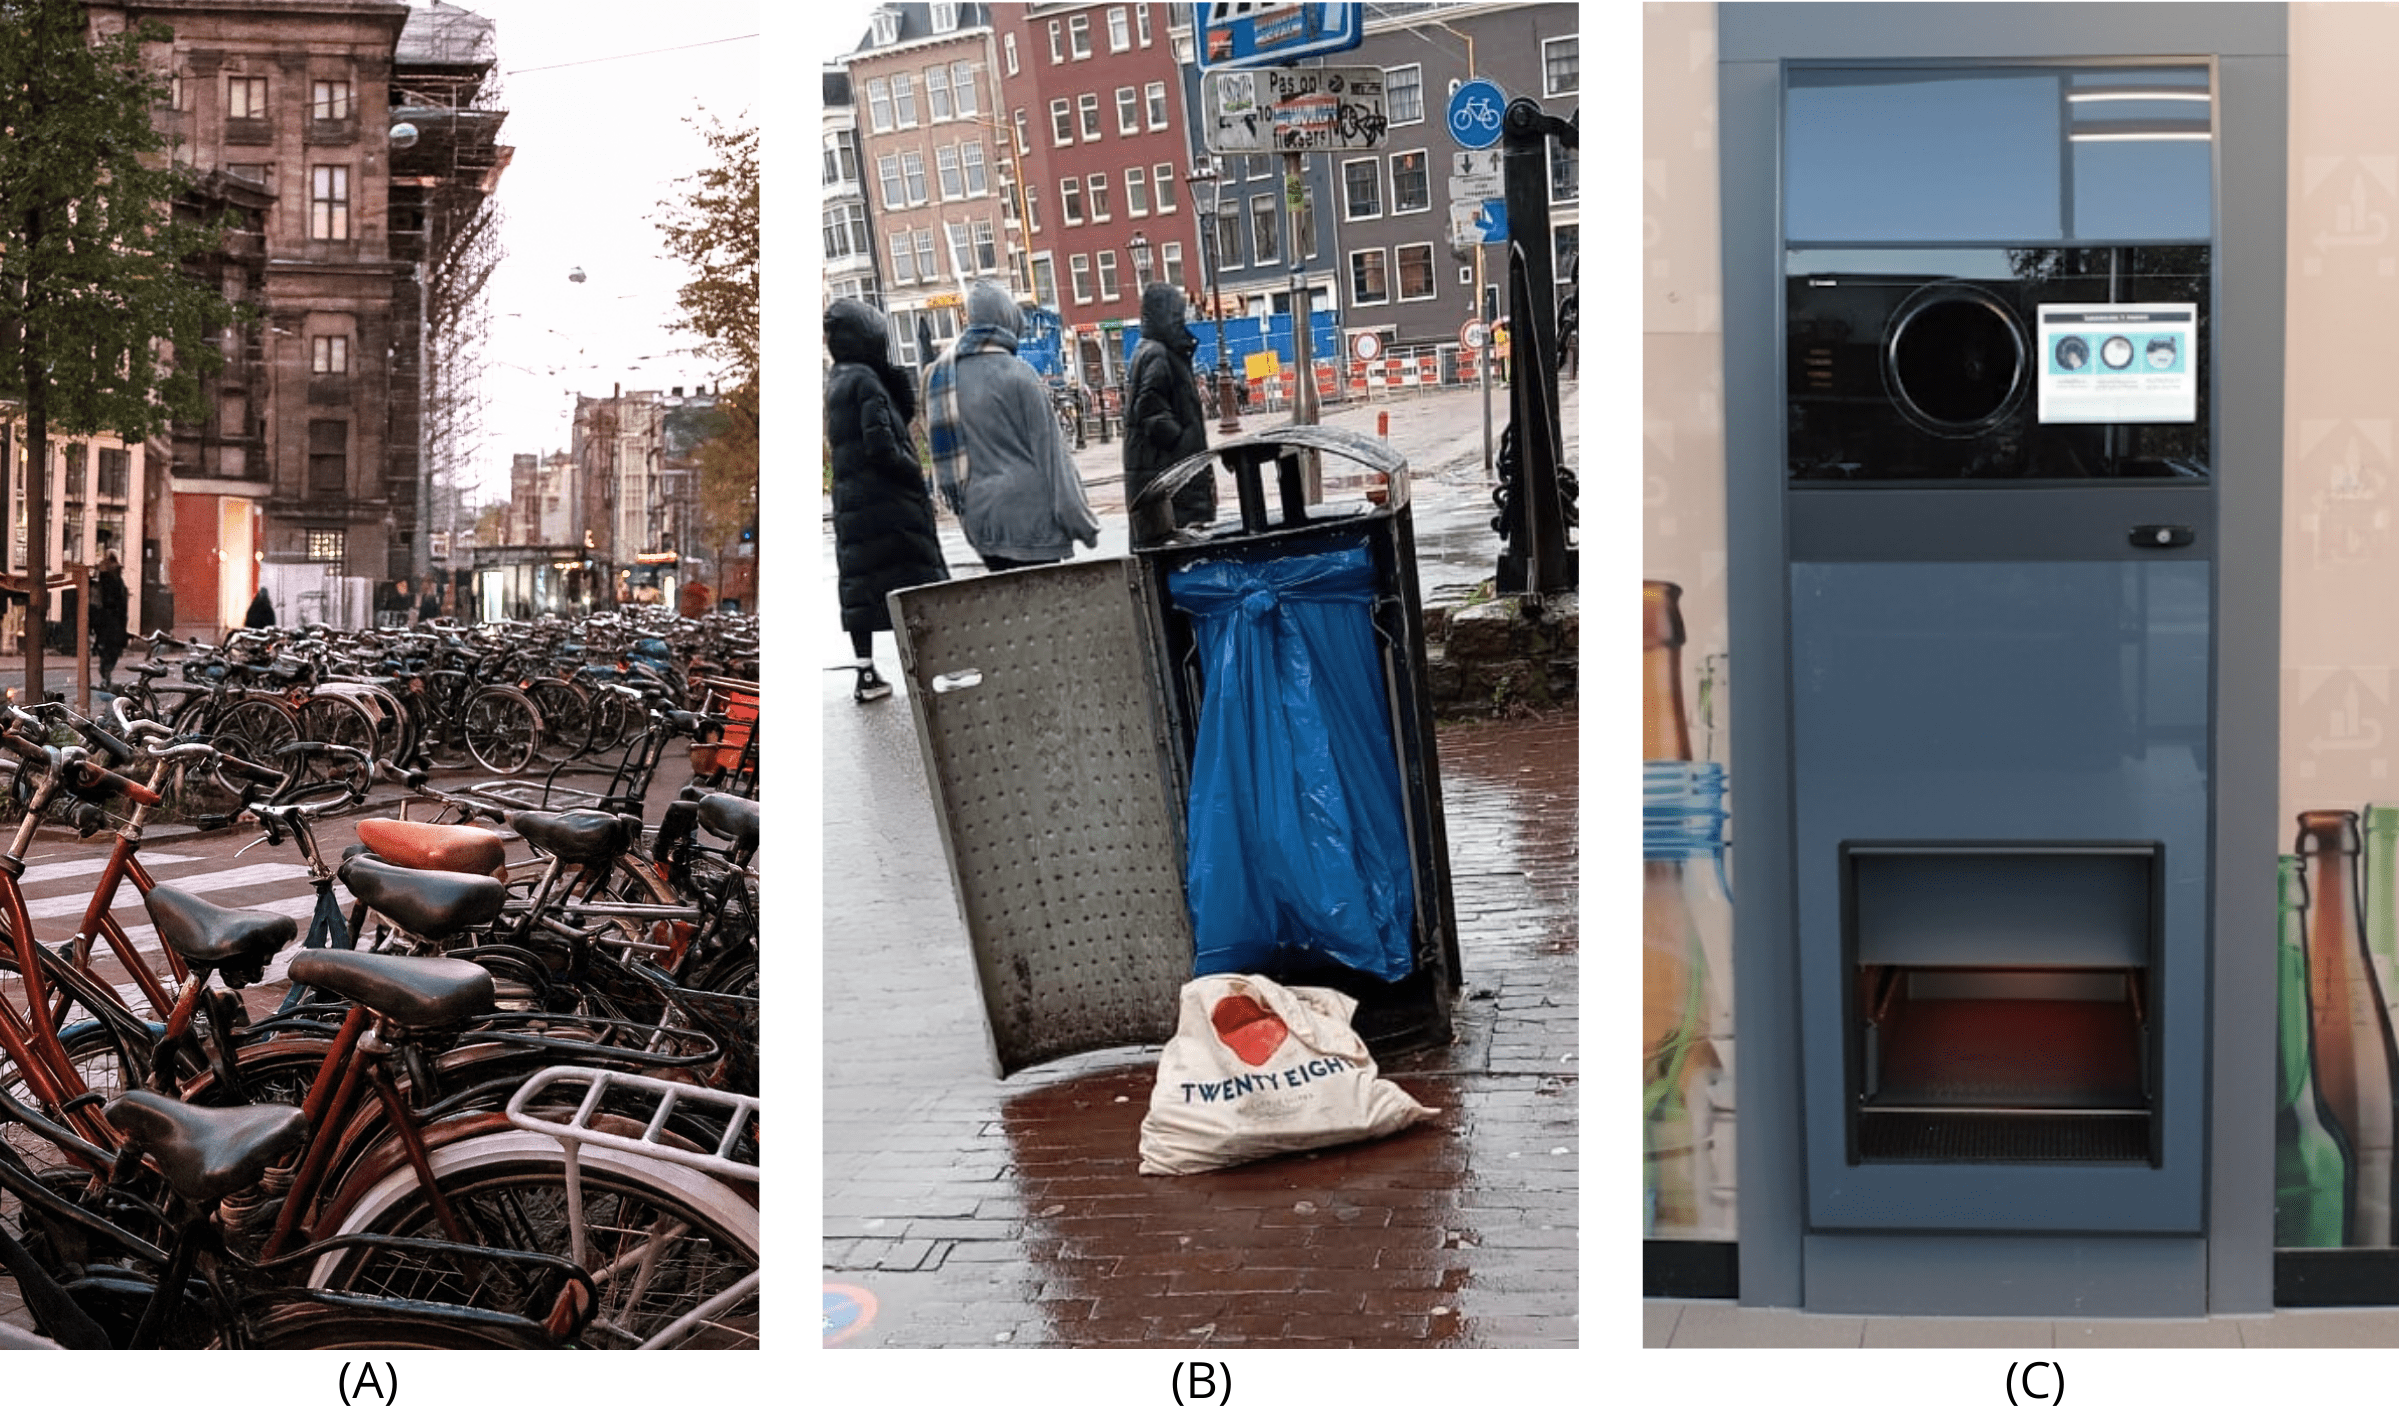
\includegraphics[width=\linewidth]{Figures/europe-pictures.png}
	\caption{Imágenes capturadas durante el viaje de investigación a Europa}
	\label{fig:europe-pictures}
\end{figure}

\begin{figure}[!htb]
	\centering
	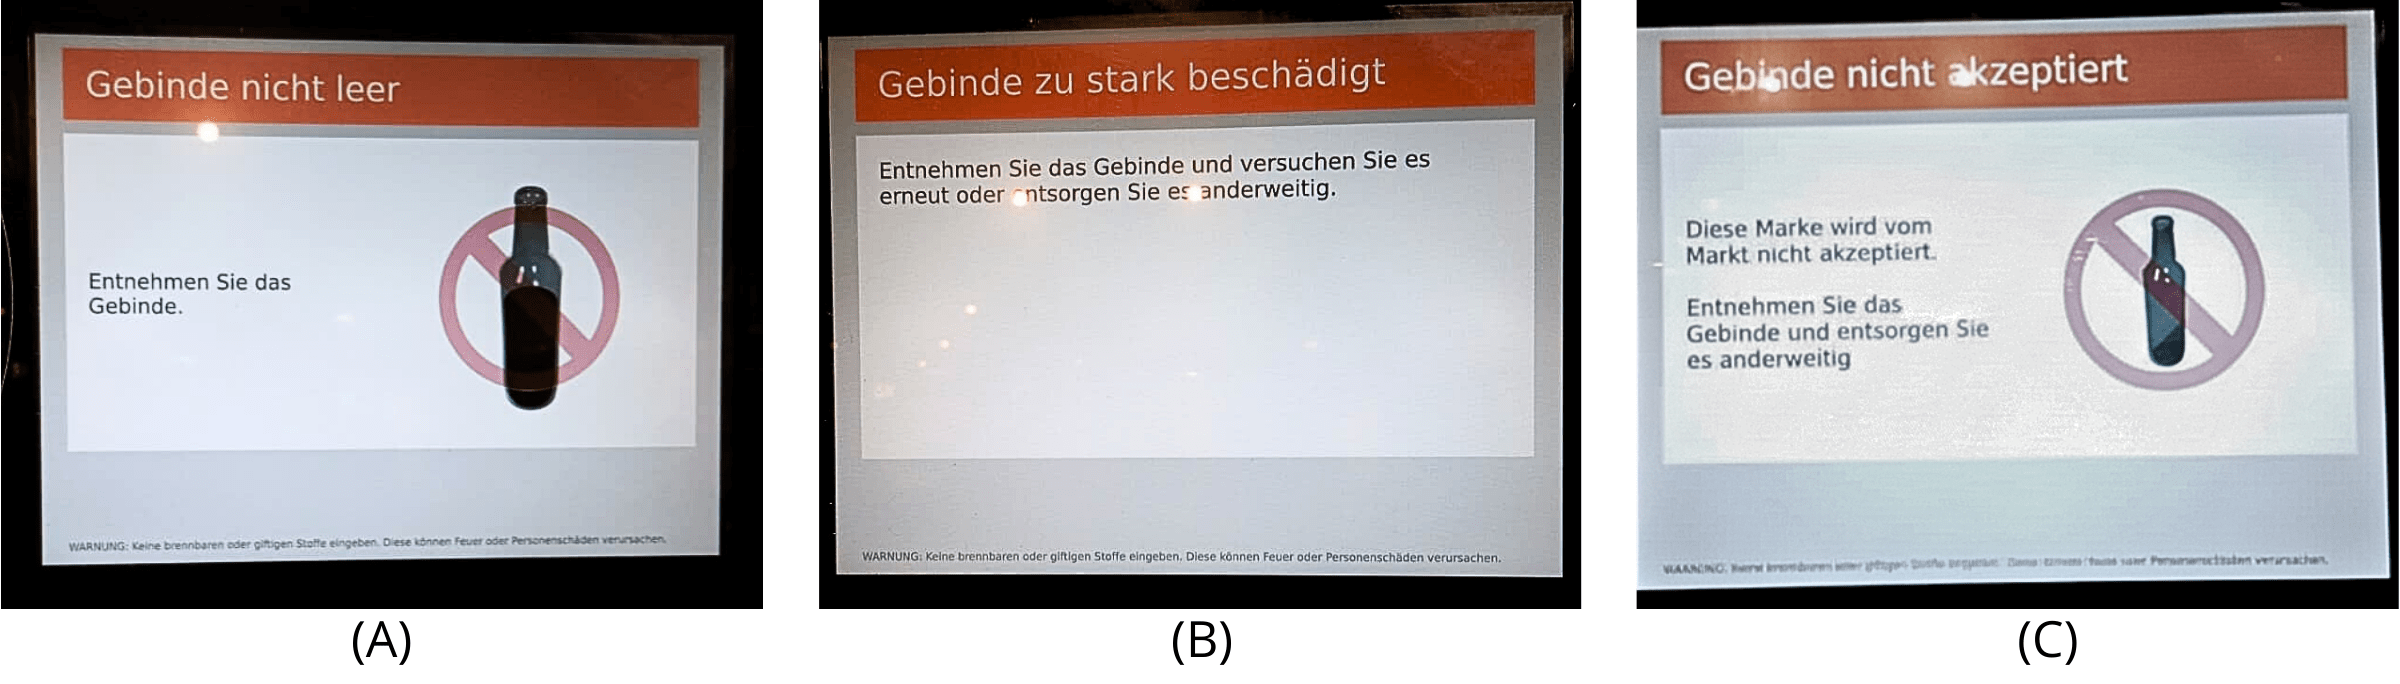
\includegraphics[width=\linewidth]{Figures/europe-pfand-cases.png}
	\caption{Mensajes asociados a casos de uso inválidos del sistema de depósito en Alemania}
	\label{fig:europe-pfand-cases}
\end{figure}
